\documentclass[a4paper,12pt]{article} % format of document

\usepackage[english,russian]{babel} % add eng,rus(base) package
\usepackage[T1,T2A]{fontenc}        % add eng,rus encoding support
\usepackage[utf8]{inputenc}         % add UTF8 support
\usepackage{soul}         	    % add l a t e r s p a c i n g
\usepackage{longtable}         	    % To display tables on several pages
\usepackage{booktabs}         	    % For pretter tables
\usepackage{enumitem}         	    % advanced list support

\usepackage{amsmath, amsfonts, amssymb, amsthm, mathtools} % add math support

\usepackage{geometry}  % add document's fields correction support
\geometry{top=25mm}    % top field
\geometry{bottom=30mm} % bottom field
\geometry{left=20mm}   % left field
\geometry{right=20mm}  % right field

\linespread{1}               % length between str
\setlength{\parindent}{20pt} % red str
\setlength{\parskip}{12pt}   % length between paragraphs

\usepackage[backend=biber, style=authoryear-icomp]{biblatex} % add bibliography support
\addbibresource{$HOME/latex-templates/biblio.bib}            % path to bibliography base
\usepackage{csquotes}                                        % advanced facilities for inline and display quotations

\usepackage{indentfirst} % first paragraph with red str

% Must be the last command into the preamble of document.
\usepackage{hyperref} % All references in document turn into hyperlinks
\hypersetup{
unicode=true,      % юникод в названиях разделов pdf
colorlinks=true,   % цветные ссылки вместо ссылок в рамках
linkcolor=blue,    % внутренние ссылки
citecolor=green,   % ссылки на библиографию
filecolor=magneta, % ссылки на файлы
urlcolor=blue,     % ссылки на url
}
 % here is document's settings for russian
%\input{$HOME/studyproject/universe/history/preamble-beamer-eng.tex} % here is document's settings for english


%\logo{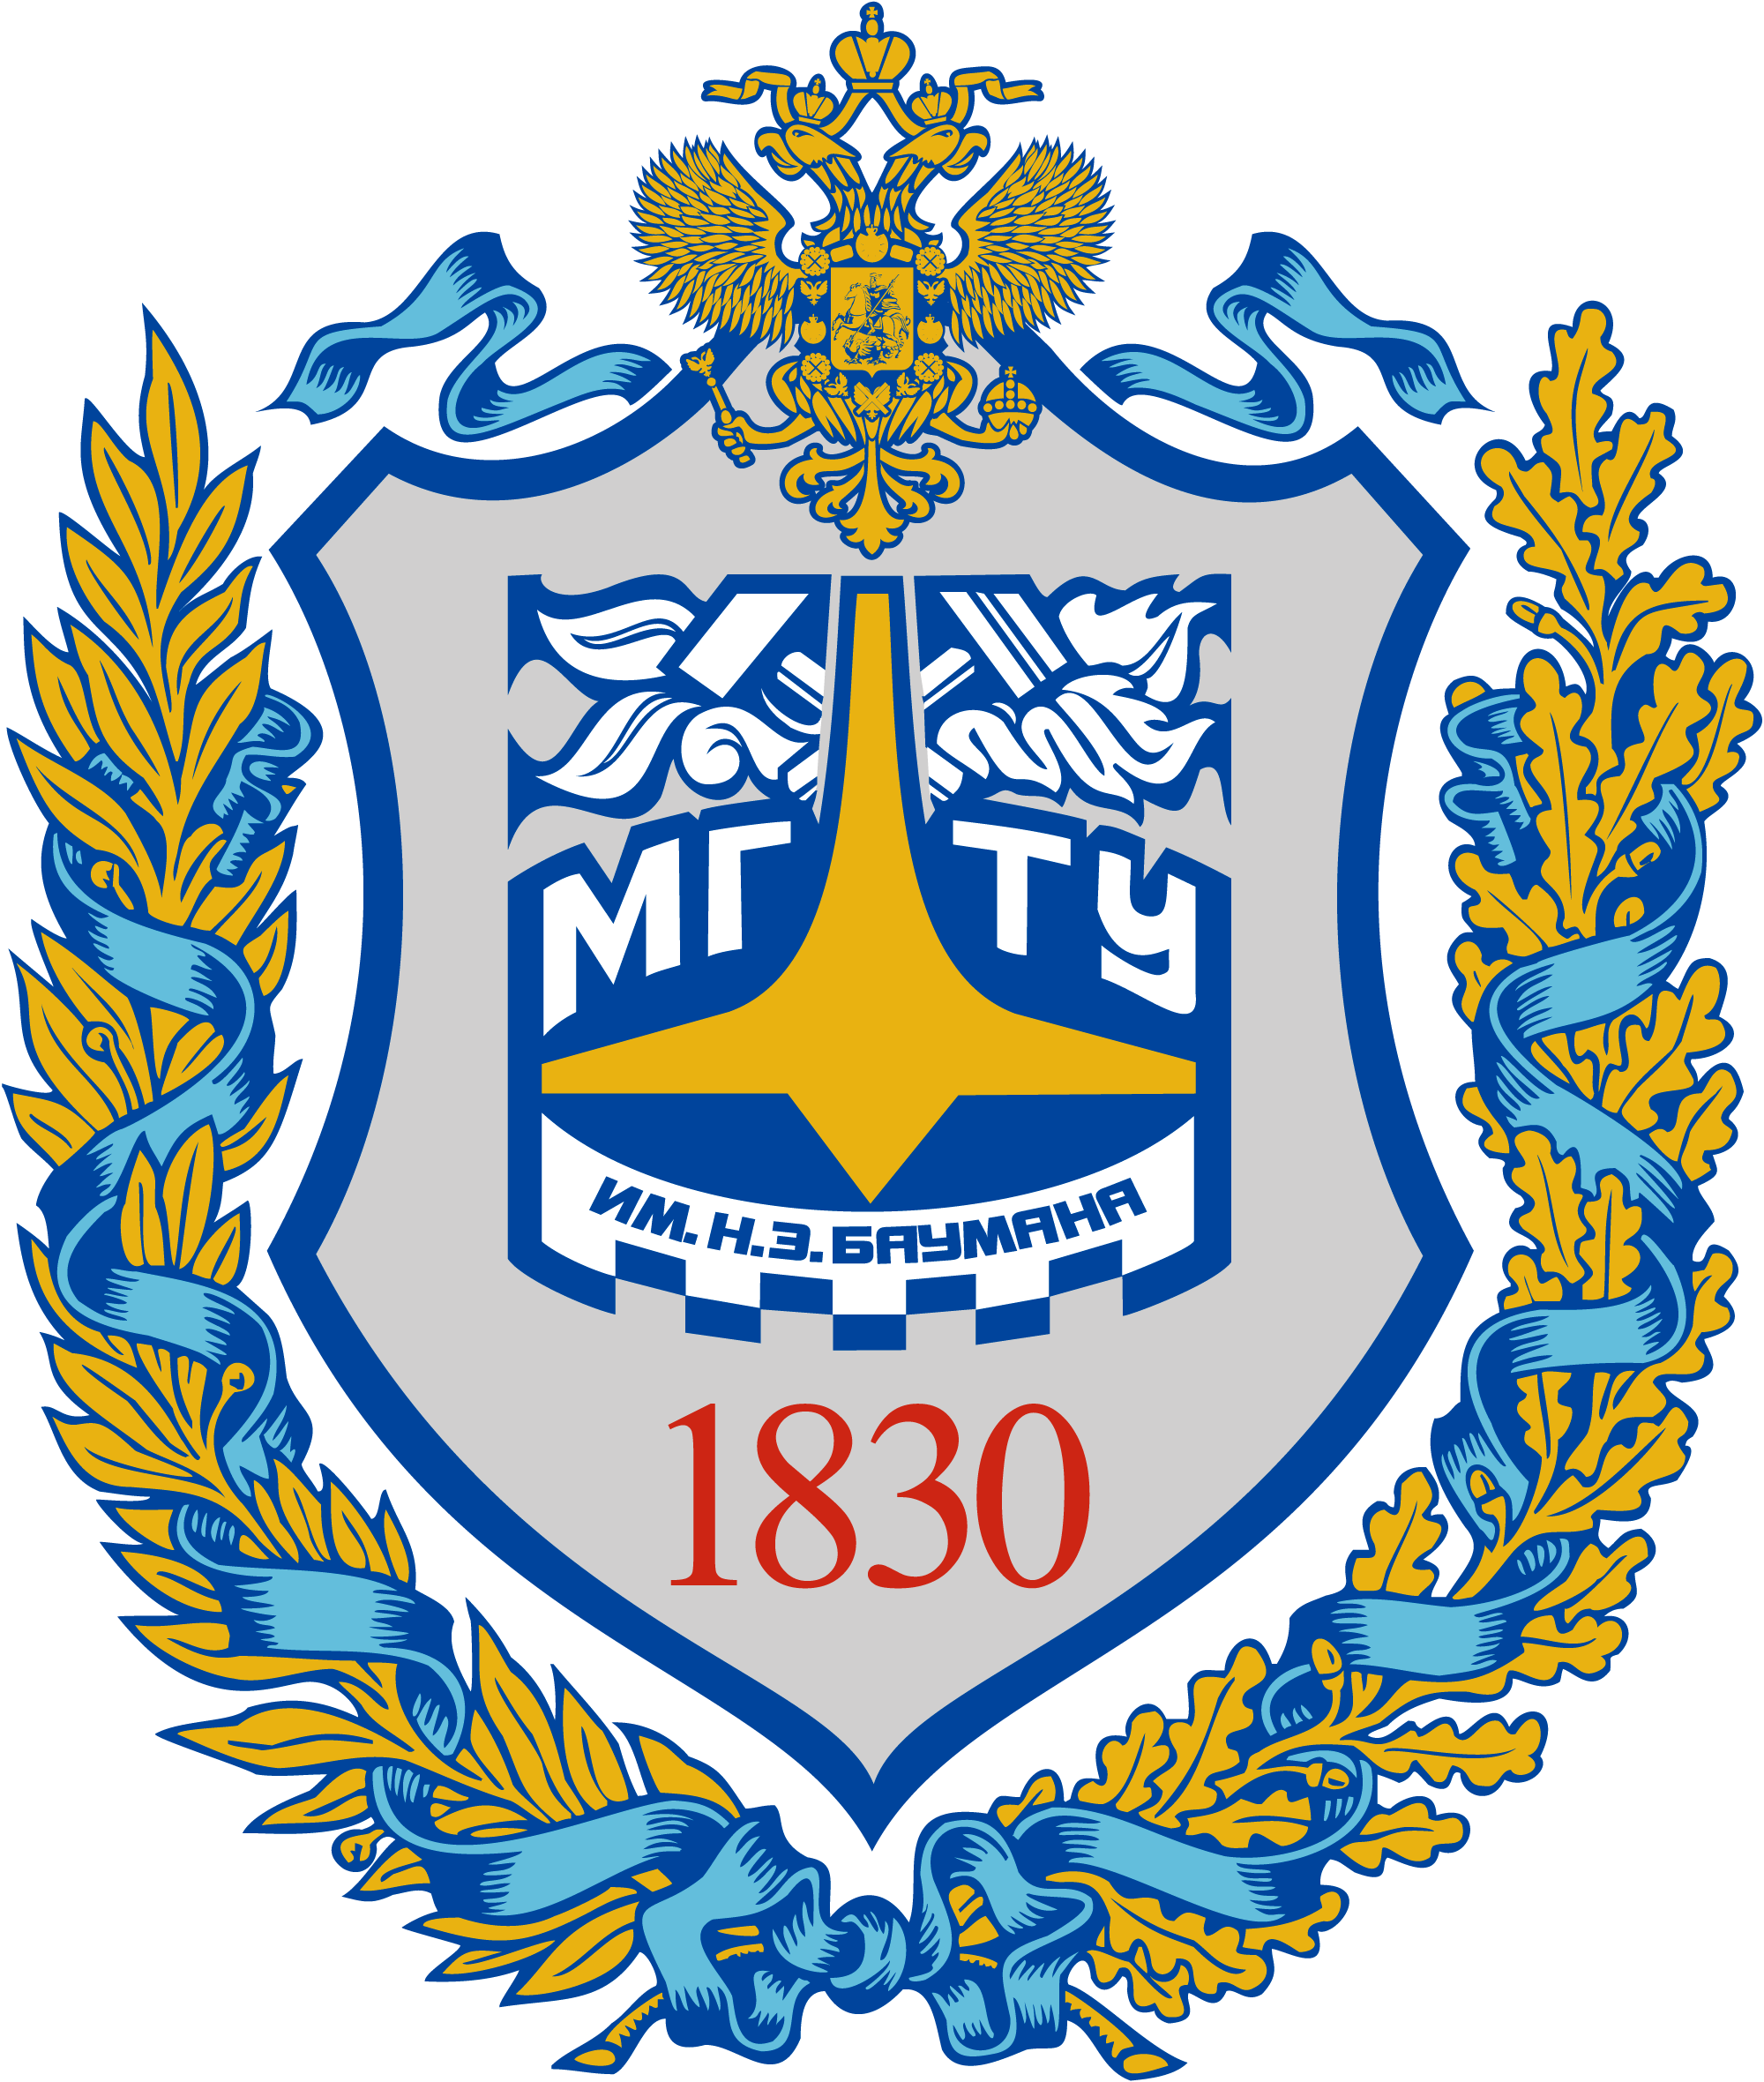
\includegraphics[width=1cm]{images/logo}}

\begin{document}

\begin{center}
	\Large{Московский Государственный Технический Университет им Н.Э. Баумана}
	\Huge{\textbf{Реферат}}

	Танк Т-72


	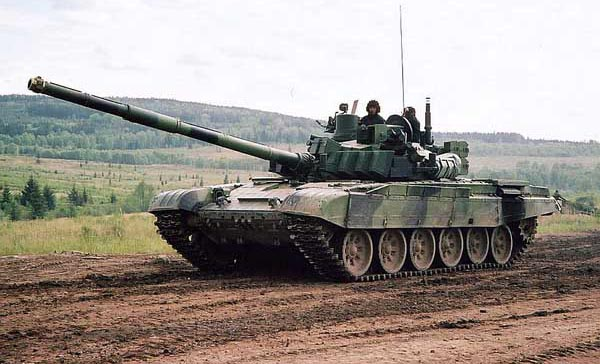
\includegraphics[width=0.9\textwidth]{images/tank1.jpg}

\end{center}
\mbox{}
\vfill
Подготовил Немков Н.М. СМ4-11
\begin{center}
Москва, 13.11.2023
\end{center}
\newpage
\tableofcontents

\newpage

Советский основной боевой танк Т-72 стал самым массовым и одним из лучших в мире, причём отнюдь не благодаря рекламе или голословным утверждениям. Он на протяжении многих лет производился и поставлялся в различные страны, где применялся с успехом, заслуживая любовь и уважение всех, кто воевал на нём или сталкивался с ним в роли врага.

Инженеры СССР всегда старались сохранить преемственность легендарного среднего танка Т-34, ставшего своеобразным символом победы над фашизмом и зарекомендовавшего свою конструкцию как дешёвую и неприхотливую. Именно он положил начало массовым и простым танкам, которые, несмотря на свою доступность, обладали всеми требуемыми характеристиками и были способны бороться на равных с лучшими образцами западных машин, а в чём-то и превосходили их.

\section{Создание}
	 Т-72 эпохи Холодной войны не стал исключением из правил и был создан как простая, надёжная и неприхотливая боевая машина, которая способна на равных конкурировать с любым другим вражеским танком. То, что ОБТ удался, подтверждает количество произведенных экземпляров, составившее более 30000 и уступившее лишь Т-54/55.

Изначально создавался Объект 172, который постепенно развился в Объект 172М, поступивший в производство под названием Т-72. 7 августа 1973 года он был принят на вооружение решением ЦК КПСС и Совета Министров СССР, после чего производился в нашей стране с 1974 по 1992 годы


\section{Особенности конструкции}

	Внешность и конструкция в целом нового Т-72 соответствовали привычной советской концепции, которая подразумевала сбалансированное сочетание подвижности, огневой мощи и защиты. Его силуэт был низок и малозаметен с любой стороны, а броня имела большие углы наклона. Гладкоствольная 125 миллиметровая пушка могла поражать любые цели того времени, а карусельный автомат заряжания уменьшал количество членов экипажа до трёх, размеры танка и поднимал скорострельность, позволяя при этом произвольно выбирать тип снаряда по приказу командира.

	Также танк получил ковш под нижним бронелистом, позволяющий проводить некоторые инженерные работы.



\section{Вооружение}

	Главное орудие представляло собой 125 миллиметровую гладкоствольную пушку Д-81ТМ (2А46), имеющую специальную конструкцию, позволяющую менять ствол прямо в полевых условиях, не демонтируя само орудие. В боекомплекте главного орудия подкалиберные, кумулятивные и осколочно-фугасные снаряды. Возможен запуск ракет управляемого типа — «Свирь». Боекомплект размещался в разных местах. В автомате заряжания карусельного типа, находилось 22 снаряда, а оставшиеся 23 снаряда были уложены в немеханизированных боеукладках корпуса и башни.

\centering

\begin{tabular}{ccc}

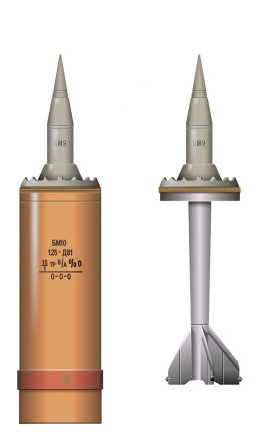
\includegraphics[width=0.3\textwidth]{images/boecom1} &

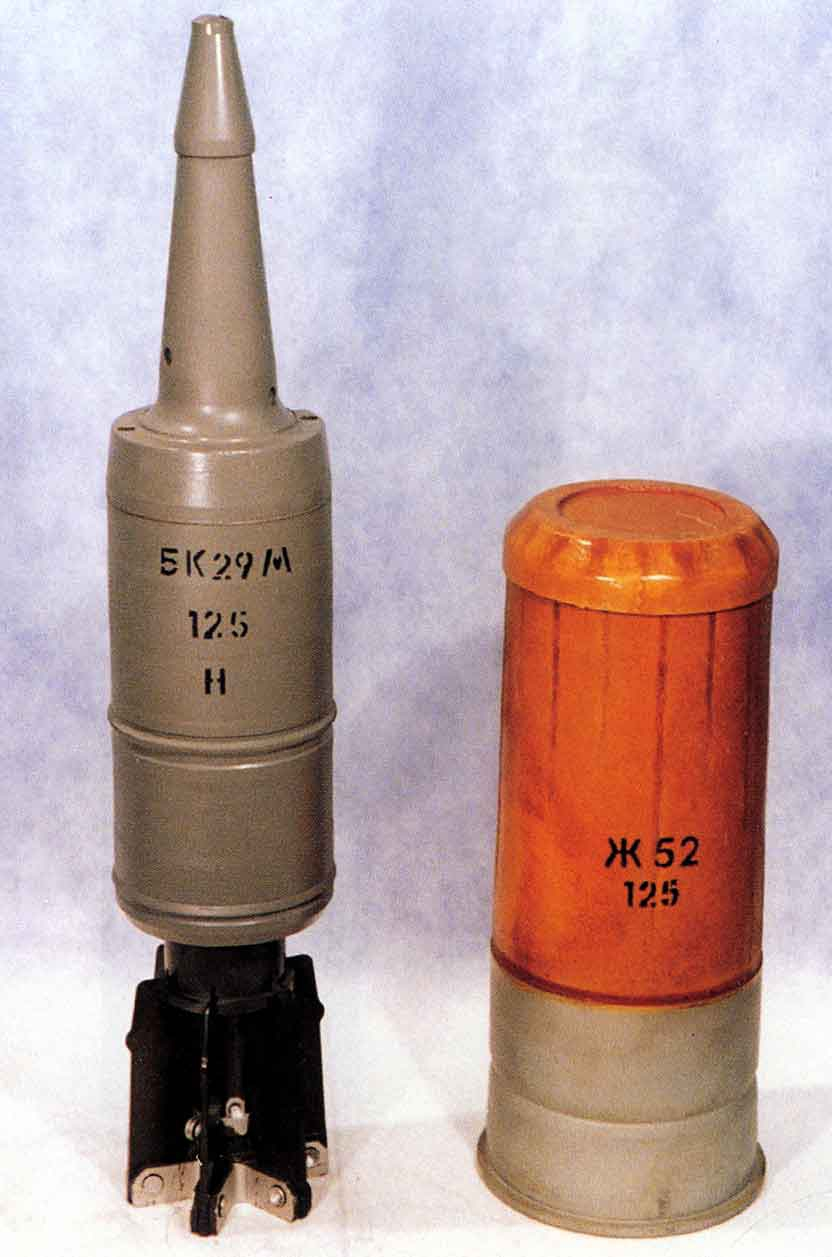
\includegraphics[width=0.3\textwidth]{images/boecom2} &

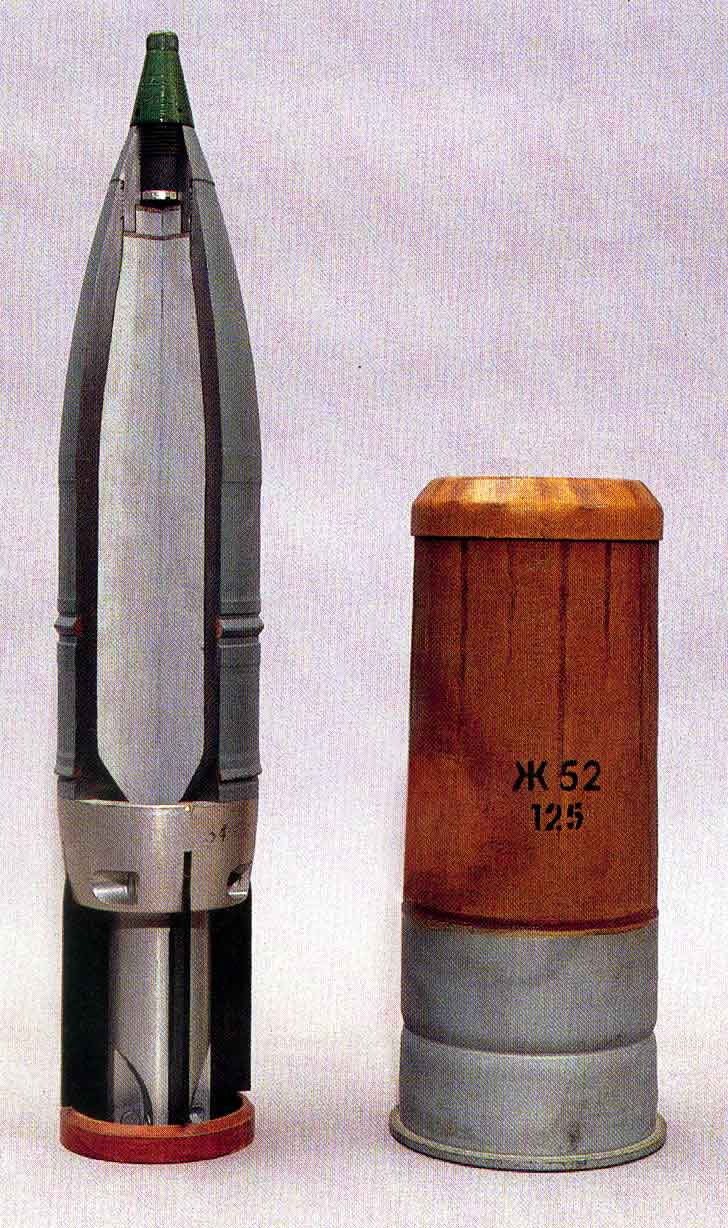
\includegraphics[width=0.3\textwidth]{images/boecom3} \\

подкалиберные &
кумулятивные &
осколочно-фугасные \\

\end{tabular}

Дополнительное вооружение состояло из двух пулемётов разного калибра. 7,62 миллиметровый пулемёт ПКТ с боекомплектом 2000 патронов был спарен с пушкой, а зенитный 12,7 миллиметровый пулемёт НСВТ находился на крыше башни и имел боекомплект в 300 патронов.

Позже были добавлены дымовые гранатомёты на борта башни, для самостоятельного создания дымовых завес.


\section{Подвижность}

	В движение ОБТ приводил привычный для СССР многотопливный дизельный двигатель. На первых модификациях был установлен 12 цилиндровый В-84-1 с жидкостным охлаждением и наддувом. Его мощность достигала 840 л.с. при 2000 об/мин.

Свой момент он передавал на механическую коробку передач с гидроприводом, имеющую семь ступеней хода вперёд и одну назад. Так же она обеспечивала поворот танка.

Ходовая часть Т-64 была признана неудачной, поэтому на Т-72 она состояла из 6 опорных катков большого диаметра, 3 поддерживающих маленького, направляющего колеса спереди и ведущего сзади.

Т-72 отличался неплохой подвижностью на любой местности и развивал 60 км/час при езде по шоссе и 35 км/час при езде по пересечённой местности.

Топливная система имела четыре внутренних бака в забронированном объёме и пять наружных топливных бака, расположенных на правой надгусеничной полке. Ёмкость внутренних баков достигала 705 литров, тогда как наружных — 495 литров. Кроме этого, на затяжных маршах можно было подключать два дополнительных бака, крепящихся на корме и имеющих объем до 500 литров. Всё это давало дальность хода 500 километров, а с установленными внешними баками до 700 километров.

Современная модификация Т-72Б3 с мощным новым двигателем обладает отличной подвижностью, позволяющей завоёвывать первые места на танковых марафонах.

\section{Бронезащита}
	Броня корпуса создавалась сильно дифференцированной, комбинированного типа. Верхняя лобовая деталь представляла собой лист трёхслойной комбинированной брони, состоящий из 80 мм стального наружного, 105 мм среднего стеклотекстолитового и 20 мм стального внутреннего слоёв. Этот лист располагался под углом в 68 градусов, благодаря чему его приведённая толщина достигала 550 мм. Нижняя лобовая деталь - лист обычной катанной гомогенной броневой стали толщиной 85 мм под углом 60 градусов.

Борта корпуса, расположенные вертикально, имели толщину 80 мм в области обитаемого объема и 70 мм в области моторно-трансмиссионного отсека.

Так же на боках корпуса имелись противокумулятивные бортовые экраны, состоящие из алюминиевого сплава, которые в походном состоянии можно было складывать, прижимая к пылевым щиткам для того, чтобы избежать случайных повреждений.

Башня изначально создавалась и производилась с монолитным бронированием, что большинство считало главным и наиболее критичным недостатком ОБТ, поэтому в 1979 году на модификации под обозначением Т-72А была установлена башня с комбинированной современной бронезащитой.

Так же у всех современных модификаций лобовые и боковые части корпуса с башней имеют дополнительную навесную или встроенную динамическую защиту.

\section{Производство и модификации}

	ОБТ производился в Индии, Ираке, Польше и Чехословакии во времена СССР, а, после его распада, в Индии, Иране и Польше, чем и заслужил свою известность.

Более того, было произведено огромное количество модификаций в различных странах, начиная от довольно привычных , вроде установки своего оборудования, заканчивая оригинальными вроде индийского Tank EX, представляющего из себя башню от Арджун на шасси Т-72.
Танк Т-72

Т-72 Урал был создан в 1973 году и представлял из себя простой Т-72.

Т-72А первая значительно изменённая версия, была выпущена в 1979 году и имела новые системы наведения и наблюдения, пушку 2А46М вместо 2А26М2, системы защиты экипажа, дымовые гранатомёты, сплошные противокумулятивные экраны на бортах и двигатель В-46-6.

Т-72АВ и Т-72Б были выпущены в 1985 году, первая из них получила навесную динамическую защиту, а вторая модификация комплекс управляемого вооружения.

Т-72БА появились в результате модернизации и доведения до уровня современных ОБТ поступивших для ремонта в 1999 году Т-72Б на УралВагонЗавод. Они получили встроенную динамическую защиту, систему управления огнём с датчиком ветра и новые двигатель с трансмиссией.

Т-72Б3 это самая последняя версия, начавшая поставляться в 2011 году на вооружение армии России, имеющая новые систему управления огнём, ДЗ Контакт-5, двигатель В-84-1 мощностью 840 л.с, ходовую, автомат заряжания и боеприпасы. С 2014 года на неё устанавливается другой двигатель, мощностью 1130 л.с., что ещё больше подняло подвижность.

ОБТ использовался более чем в 40 армиях, начиная от времени своего производства, заканчивая современностью. В наше время он весьма распространён, а то, что российский основной боевой танк Т-90 является по сути его глубокой модификацией, говорит о многом.

    \begin{center}
	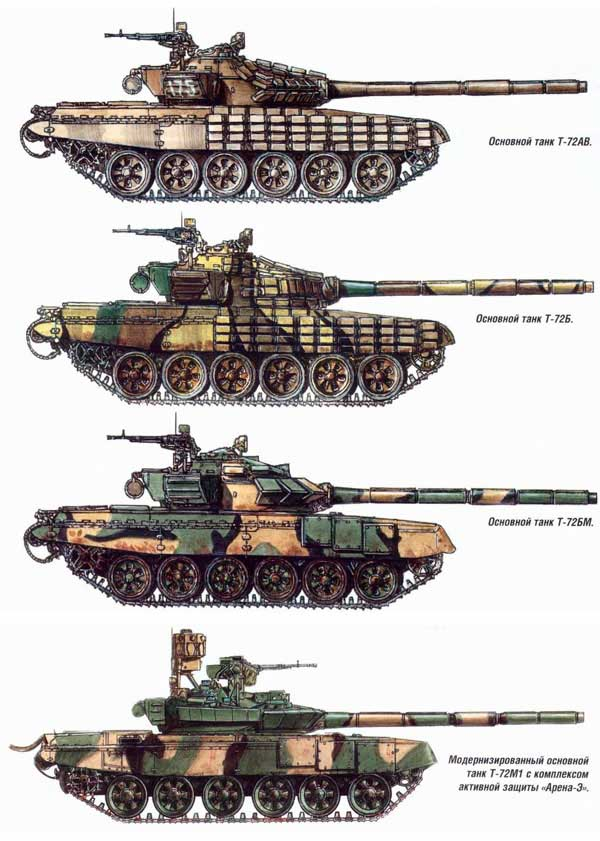
\includegraphics[width=0.5\textwidth]{images/tank2.jpg}
    \end{center}

\section{Боевое применение}

	Впервые танк применили при боевых действиях в 1982 году в Ливане, в долине Бекаа. Две сирийские танковые бригады попали в окружение и было принято решение отправить им на помощь элитную бригаду, оснащённую новыми Т-72. Они успешно уничтожили несколько израильских М60, практически не понеся потерь, прорвав тем самым окружение.

В Ираке советские машины проявили себя ещё лучше, практически без достойного сопротивления уничтожая Чифтены и Скорпионы, а всего за 8 лет войны, было потеряно 60 танков.
Танк Т-72

А вот во время вторжения в Кувейт, где советским ОБТ противостояли американские Абрамс М1А1 новой модификации, оснащённые 120 миллиметровой немецкой пушкой, было потеряно до 250 Т-72. Более того, известен случай, когда увязший в грязи Абрамс был атакован 3 Т-72, уничтожил их, и был отбуксирован на базу, после чего вновь вступил в строй.

Такое соотношение потерь можно объяснить отсутствием современных снарядов, способных справиться с бронёй Абрамса, у Ирака.

В Грузии, Чечне и Осетии Т-72 опять понесли большие потери, причём в Осетии обе стороны конфликта были вооружены ими, но Россия потеряла 2 танка, а Грузия 18, что доказывает то, что все эти потери произошли лишь из-за плохой подготовки экипажей и неправильного командования.

Действительно, во время штурма Грозного, танки применялись без прикрытия стрелков в городских условиях и уничтожались выстрелами в борта и корму, при этом случаи пробития лобовой брони неизвестны.

Были отмечены надёжность на марше в горных условиях и способность выдерживать многочисленные попадания без заметных повреждений.

\section{Характеристики}

\begin{center}
\begin{tabular}{ccc}
	Основные & характеристики \\
	Страна & СССР \\
	Принят на вооружение & 1973 \\
	Экипаж & 3 \\
	Масса &	46 т \\
	Длина с орудием & 9.53 м \\
	Длина корпуса & 6.67 м \\
	Ширина & 3.59 м \\
	Высота & 2.19 м \\
	Вооружение Главное орудие & 125 мм 2А46М / 2А46М-5 \\
	Пулемёт & 12,7 мм НСВ, 7,62 мм ПКТМ \\
	Углы склонения орудия & -6 +13 \\
	Боекомплект орудия & 39 \\
	Боекомплект пулемёта & 2000 патронов 7,62 мм, 300 патронов 12,7 мм \\
	Подвижность Двигатель & B-92C2 \\
	Мощность & 1000 л.с \\
	Максимальная скорость по шоссе & 65 км/ч \\
	Запас хода & 500 км \\
	Преодолеваемый подъём & 30 ° \\
	Преодолеваемая стенка & 0.85 м \\
	Преодолеваемый ров & 2.8 м \\
	Преодолеваемый брод & 1.2 м \\
	Преодолеваемый брод с подготовкой & 1.8 м \\
\end{tabular}
\end{center}

\section{Эпилог}

	За всё время было создано очень много машин на базе Т-72 - различные инженерные машины, самоходные пушки, боевые машины поддержки и опытные образцы танков.

Будучи принятым на вооружение в 1973 году, Т-72 сейчас стоит на вооружении многих стран, а, благодаря модификациям и современному оборудованию, способен наравне бороться со многими другими современными ОБТ и ещё долго останется в российской армии, даже после поступления в неё Т-14 Армата.

Его высокие подвижность, огневая мощь и защита вместе с надёжностью, неприхотливостью и стоимостью очень удачно собраны в одно целое, что ценится специалистами всего мира, многие из которых по праву считают Т-72 лучшим основным боевым танком второй половины 20 века.

\section{Патент}

    \begin{center}
	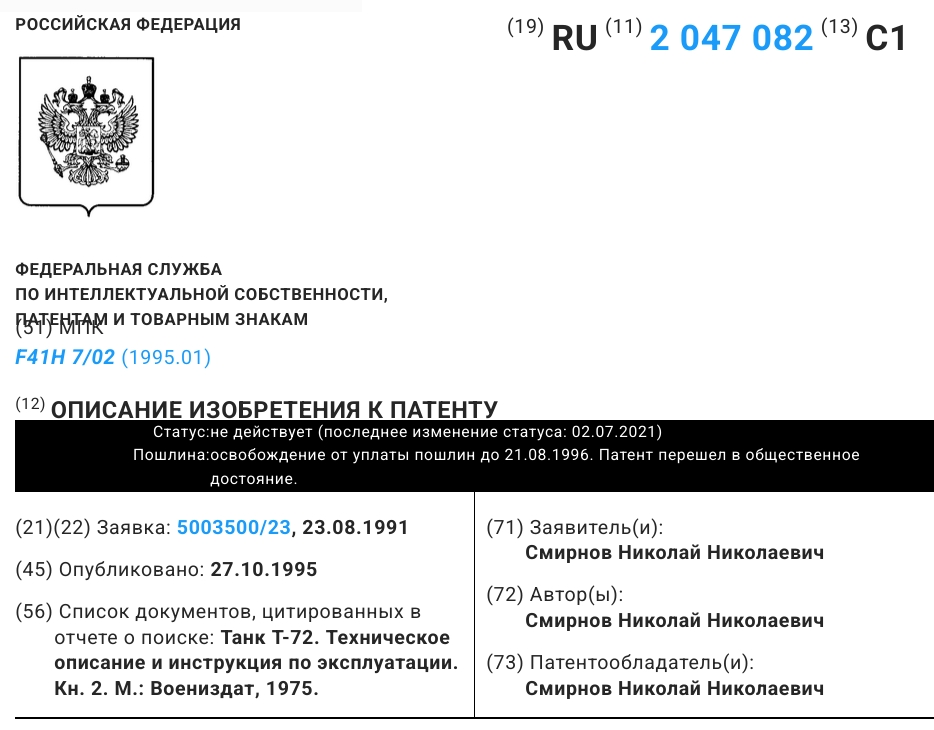
\includegraphics[width=1\textwidth]{images/tank3.jpg}
    \end{center}

    (54) ТАНК

(57) Реферат:

Изобретение относится к бронетанковой технике, а именно к танкостроению. Технической задачей изобретения является обеспечение повышенной защищенности экипажа и агрегатов танка от боевых повреждений. Танк содержит броневой корпус 1, поворотную башню 2, образующую с выполненным за одно целое с ней боксом 3 объем, в который смонтированы различные комплексы, в том числе вооружение с казенной частью орудия 4, а также места размещения экипажа. В передней части броневого корпуса 1 перед органами управления установлен бокс, выполненный в виде кресла-ложемента. В задней части броневого корпуса 1 расположена силовая двигательная установка 6, соединенная через коробку передач с ходовой частью, ведущие колеса 7 которой с каждой стороны через гусеничные ленты связаны с направляющими колесами и катками 8. Для увеличения жесткости крепления поворотной башни 2, имеющей опору в верхней части броневого корпуса 1, нижняя часть бокса 3, выполненного за одно целое с поворотной башней 2, дополнительно установлена на радиальной и осевой опорах, смонтированных в днище 12 броневого корпуса 1. Вращение поворотной башни 2 с боксом 3 осуществляется как с помощью ручного, так и механического приводов. 4 ил. [Увеличенное изображение (открывается в отдельном окне)]

Изобретение относится к бронетанковой технике, а именно к танкостроению.

Известен танк Т - 72 , содержащий броневой корпус с расположенными в нем силовой установкой, соединенной через силовую передачу с ходовой частью, органы управления, поворотную башню с оружием, выполненную за одно целое с боксом для размещения экипажа и бокс механика-водителя, размещенный перед органами управления. ( Танк Т - 72 . Техническое описание и инструкция по эксплуатации. Кн.2, М. Воениздат, 1975)
Недостатком этого танка является недостаточная живучесть при поражении противотанковыми средствами.

Технической задачей изобретения является обеспечение повышенной защищенности экипажа и агрегатов танка от боевых поражений.

Это достигается тем, что в танке , содержащем броневой корпус с расположенной в нем силовой установкой, соединенной через силовую передачу с ходовой частью, органы управления, поворотную башню с оружием, выполненную за одно целое с боксом для размещения экипажа, и бокс механика-водителя, размещенный перед органами управления, нижняя часть башни с боксом смонтирована по периферии на радиальной и осевой опорах качения, закрепленных в днище броневого корпуса, а бокс механика-водителя, размещенный перед органами управления в передней части корпуса, имеет форму кресла-ложемента и установлен с возможностью автономного вращения.

На фиг. 1 изображен танк с разрезом его поворотной башни-бокса, вид сбоку; на фиг.2 то же, с разрезом бокса механика-водителя; на фиг.3 разрез А-А на фиг.1; на фиг.4 разрез Б-Б на фиг.1.

Танк содержит броневой корпус 1, поворотную башню 2, образующую с выполненным за одно целое с ней боксом 3 объем, в котором смонтированы различные комплексы, в том числе вооружение с казенной частью орудия 4, а также места размещения экипажа. В передней части броневого корпуса 1 перед органами управления установлен бокс 5, выполненный в виде кресла-ложемента. В задней части броневого корпуса 1 расположена силовая двигательная установка 6, соединенная через коробку передач с ходовой частью, ведущие колеса 7 которой с каждой стороны через гусеничные ленты связаны с направляющими колесами и катками 8. Для увеличения жесткости крепления поворотной башни 2, имеющей опору 9 в верхней части броневого корпуса 1, нижняя часть бокса 3, выполненного за одно целое с поворотной башней 2, дополнительно установлена на радиальной опоре 10 и осевой опоре 11, смонтированных в днище 12 броневого корпуса 1. Вращение поворотной башни 2 с боксом 3 осуществляется как с помощью ручного, так и механического приводов.

Предложенный танк , оснащенный боксами, по сравнению с известным, обладает повышенной защищенностью от средств поражения за счет выполнения поворотной башни за одно целое с боксом, за счет повышения жесткости крепления в дополнительной опоре.

Формула изобретения

ТАНК , содержащий броневой корпус с расположенной в нем силовой установкой, соединенной через силовую передачу с ходовой частью, органы управления, поворотную башню с орудием, выполненную за одно целое с боксом для размещения экипажа, бокс механика-водителя, размещенный перед органами управления, отличающийся тем, что нижняя часть башни с боксом смонтирована по периферии на радиальной и осевой опорах качения, закрепленных в днище броневого корпуса, а бокс механика-водителя, размещенный перед органами управления в передней части корпуса, имеет форму кресла-ложемента и установлен с возможностью автономного вращения.

[Увеличенное изображение (открывается в отдельном окне)] [Увеличенное изображение (открывается в отдельном окне)] [Увеличенное изображение (открывается в отдельном окне)]

ИЗВЕЩЕНИЯ

MM4A - Досрочное прекращение действия патента Российской Федерации на изобретение из-за неуплаты в установленный срок пошлины за поддержание патента в силе

Извещение опубликовано: 20.06.2000БИ: 17/2000

\end{document}
